\paragraph{Sơ đồ tuần tự luồng xử lý tài liệu trong nền}

Luồng nghiệp vụ này mô tả
phần xử lý bất đồng bộ sau khi
dịch vụ tài liệu đã gửi Celery task \texttt{process\_document\_task(doc\_id)} vào RabbitMQ.
Worker nhận công việc, tải file gốc từ R2, trích xuất nội dung, tạo summary,
ghi vector chunks vào Milvus và cập nhật trạng thái tài liệu.

\subparagraph{Mô tả tổng quan}

\begin{itemize}

\item \textbf{Nhận nhiệm vụ:}
Tiến trình xử lý tài liệu nhận nhiệm vụ xử lý
một tài liệu cụ thể từ hàng đợi tin nhắn.

\item \textbf{Tải tài liệu:}
Tiến trình cập nhật trạng thái tài liệu sang đang xử lý
và tải tệp tài liệu gốc từ kho lưu trữ trực tuyến.

\item \textbf{Phân tích và tóm tắt:}
Tiến trình phân tích nội dung tài liệu và tạo phần tóm tắt,
sau đó tải các nội dung này lên kho lưu trữ trực tuyến dưới dạng các thư mục nội dung và tóm tắt riêng biệt.

\item \textbf{Tạo định danh nhúng tìm kiếm:}
Các đoạn nhỏ của tài liệu được chuyển đổi sang dạng vector nhúng
và lưu vào CSDL vector cùng thông tin người sở hữu, định danh tài liệu và tên tệp tin để phục vụ tìm kiếm.

\item \textbf{Hoàn tất xử lý:}
Khi hoàn tất, trạng thái tài liệu được cập nhật thành đã hoàn thành
kèm thông tin xác nhận đã trích xuất nội dung và tóm tắt.
Nếu xảy ra lỗi trong quá trình xử lý, trạng thái tài liệu sẽ chuyển sang thất bại.
\end{itemize}

\begin{figure}[H]
\centering
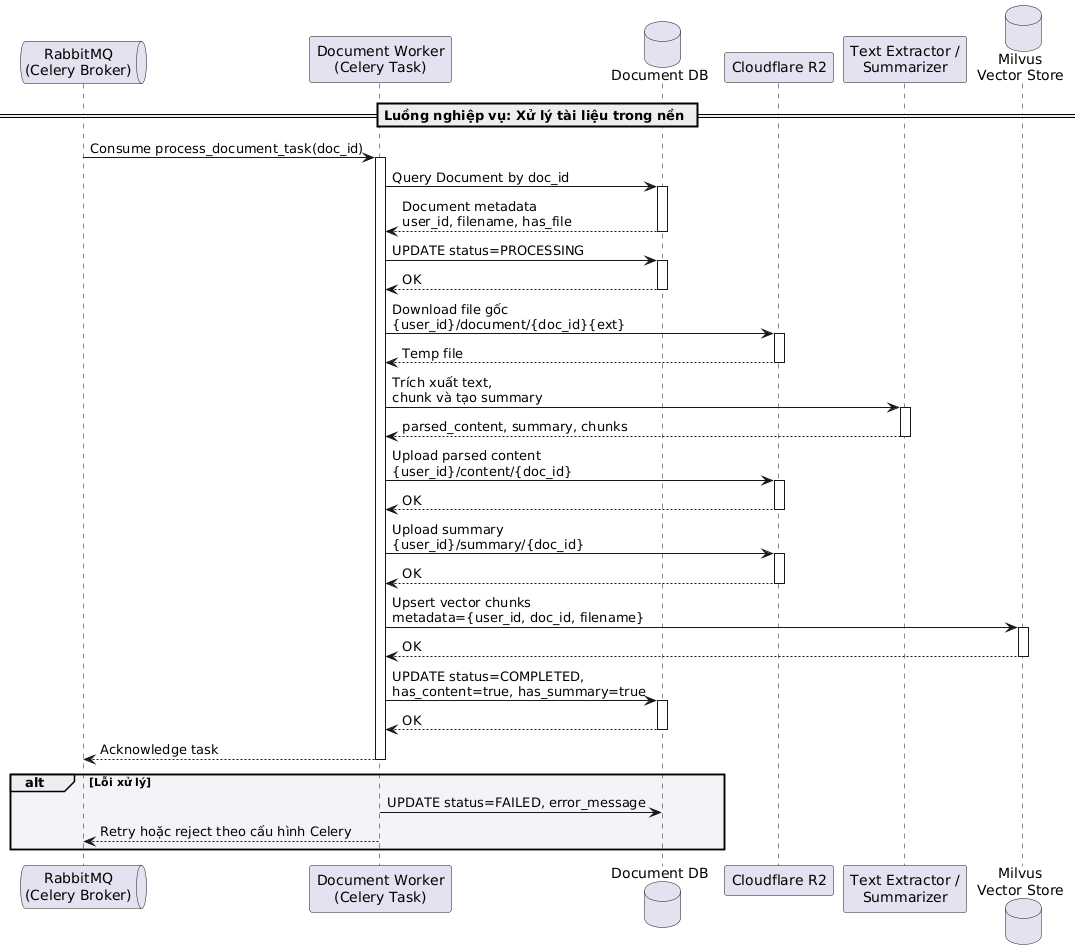
\includegraphics[width=0.9\textwidth]{contents/Sequence/UML-Sequence-DocumentWorkerProcessDocument.png}
\caption{Sơ đồ tuần tự luồng xử lý tài liệu trong nền}
\end{figure}

\begin{table}[H]
\centering
\renewcommand{\arraystretch}{1.3}

\begin{tabular}{|l|l|p{5cm}|}
\hline
\textbf{Thành phần} & \textbf{Phân loại} & \textbf{Vai trò trong hệ thống} \\ \hline
RabbitMQ & Message Broker & Phân phối Celery task xử lý tài liệu cho worker. \\ \hline
Document Worker & Background Worker & Xử lý file, cập nhật trạng thái và ghi dữ liệu phục vụ RAG. \\ \hline
Document Database & Database & Lưu thông tin xử lý tài liệu. \\ \hline
Cloudflare R2 & Object Storage & Lưu file gốc, parsed content và summary. \\ \hline
Text Extractor / Summarizer & Processing Component & Trích xuất text, chia chunk và tạo summary. \\ \hline
Milvus & Vector Store & Lưu vector chunks theo user và document để truy vấn về sau. \\ \hline
\end{tabular}
\caption{Các thành phần tham gia luồng xử lý tài liệu trong nền}
\end{table}
